\chapter{From One-Particle Quantum Mechanics to a Simple Quantum Field}

These notes follow Leonard Susskind's seventh lecture in \emph{Advanced Quantum Mechanics} and develop, from the particle side, the basic construction of a simple quantum field for a single nonrelativistic species. The lecture moves deliberately: first the motivation for allowing variable particle number, then a careful return to one-particle wavefunctions and orthonormal modes, and only afterward the passage to Fock space, field operators, density operators, and the Hamiltonian of the field. This chapter is a first-pass companion draft based on that lecture, with curation by LazyingArt LLC (\texttt{https://lazying.art}).

\section{Why Fixed Particle Number Is Not Enough}

Susskind begins by emphasizing that there are two complementary routes into quantum field theory. One may begin with fields and discover quanta, or one may begin with particles and reconstruct why fields are the right language. This lecture takes the second route.

The physical motivation is immediate. Ordinary one-particle or few-particle quantum mechanics treats a fixed number of particles, but nature does not. Photons are constantly emitted and absorbed. Unstable particles decay. A neutron can turn into a proton, an electron, and a neutrino. The total number of particles changes. If one wants a single quantum-mechanical framework that can describe such processes, one needs a formalism broad enough to include arbitrary occupation number from the outset.

For the whole lecture Susskind keeps the scope narrow. There is only one species of particle, and the dynamics are nonrelativistic. This is already enough to exhibit the central point: fields are the natural bookkeeping device for a quantum theory in which particle number is allowed to vary.

\section{One-Particle Quantum Mechanics Recalled}

Susskind next slows down and rebuilds the one-particle language from the beginning. If $|\psi\rangle$ is a one-particle state and $|x\rangle$ denotes a state localized at position $x$, then the wavefunction is
\begin{equation}
\psi(x)=\langle x|\psi\rangle.
\end{equation}
The quantity $\psi(x)$ is a probability amplitude. The probability density is therefore
\begin{equation}
|\psi(x)|^2=\psi^*(x)\psi(x),
\end{equation}
and for a normalized one-particle state,
\begin{equation}
\int dx\,\psi^*(x)\psi(x)=1.
\end{equation}

At this stage the symbol is deliberately lower-case. These are ordinary one-particle wavefunctions, not field operators. That distinction will matter later, and Susskind repeatedly insists on it.

A useful observation already appears here. In the one-particle sector the integral of $|\psi(x)|^2$ is both total probability and, trivially, the total number of particles. This coincidence ceases to be trivial as soon as we pass to many-particle states.

\section{Modes, the Particle in a Box, and Completeness}

Any orthonormal basis of one-particle states can be used, but energy eigenstates are especially convenient. Susskind illustrates this with a particle in a box. The walls of the box are represented by a sharply rising potential, and the first few energy eigenfunctions are sine-like standing waves ordered by node count.

\begin{figure}[t]
\centering
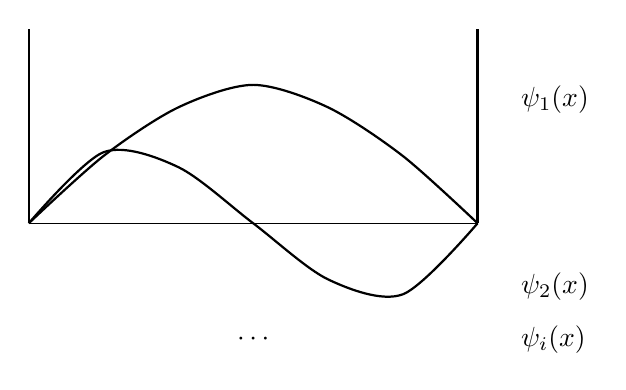
\begin{tikzpicture}[scale=0.95]
\draw[thick] (0,0) -- (0,2.6);
\draw[thick] (6,0) -- (6,2.6);
\draw[thin] (0,0) -- (6,0);

\draw[thick, smooth] plot coordinates {(0,0) (1,0.9) (2,1.55) (3,1.85) (4,1.55) (5,0.9) (6,0)};
\draw[thick, smooth] plot coordinates {(0,0) (1,0.95) (2,0.75) (3,0) (4,-0.75) (5,-0.95) (6,0)};

\node[right] at (6.45,1.65) {$\psi_1(x)$};
\node[right] at (6.45,-0.85) {$\psi_2(x)$};
\node[right] at (6.45,-1.55) {$\psi_i(x)$};
\node at (3,-1.55) {$\cdots$};
\end{tikzpicture}
\caption{A particle-in-a-box basis, drawn in the spirit of the lecture. The first modes are sine-like standing waves and are naturally ordered by node structure.}
\end{figure}

The orthonormality relation is
\begin{equation}
\int dx\,\psi_i^*(x)\psi_j(x)=\delta_{ij}.
\end{equation}
The basis is also complete:
\begin{equation}
\sum_i |i\rangle\langle i|=\mathbf{1}.
\end{equation}

\paragraph{Completeness and the delta function.}
This is the last major piece of one-particle mathematics before the transition to fields. Sandwich the resolution of the identity between position states:
\begin{align}
\langle x|y\rangle
&=\langle x|\mathbf{1}|y\rangle
=\sum_i \langle x|i\rangle\langle i|y\rangle \\
&=\sum_i \psi_i(x)\psi_i^*(y).
\end{align}
Since $\langle x|y\rangle=\delta(x-y)$, one obtains the completeness relation in position space,
\begin{equation}
\sum_i \psi_i(x)\psi_i^*(y)=\delta(x-y).
\end{equation}
Susskind emphasizes the practical meaning of this identity: any orthonormal basis gives a way of writing a delta function.

\section{Fock Space and Occupation Numbers}

Having finished the one-particle preliminaries, Susskind returns to the real goal: a quantum theory that can describe any number of particles.

\begin{definition}
For one species of particle, the many-particle Hilbert space is spanned by occupation-number states
\begin{equation}
|n_1,n_2,\ldots\rangle,
\end{equation}
where $n_i$ records how many particles occupy the one-particle mode $i$.
\end{definition}

These states do not live in the same vector space as the one-particle wavefunctions. This is an important conceptual shift. The $\psi_i(x)$ are functions; the occupation-number states are states of the full many-particle system.

To raise and lower the occupation numbers one introduces creation and annihilation operators,
\begin{equation}
a_i^\dagger,\qquad a_i.
\end{equation}
The operator $a_i^\dagger$ creates a particle in the mode $i$, and $a_i$ annihilates one. The corresponding number operator is
\begin{equation}
N_i=a_i^\dagger a_i.
\end{equation}
The vacuum state is the state with no particles at all,
\begin{equation}
|0\rangle = |0,0,\ldots\rangle.
\end{equation}

At this point the oscillator language is mostly bookkeeping. The detailed operator algebra is not developed systematically in this lecture; what matters immediately is that $a_i^\dagger$ and $a_i$ move us between states with different occupation numbers.

\section{Field Operators in Position Space}

The central move of the lecture is the introduction of the field operator. Susskind motivates it operationally rather than axiomatizing it.

\begin{definition}
The field operators are
\begin{equation}
\Psi(x)=\sum_i a_i\,\psi_i(x),
\qquad
\Psi^\dagger(x)=\sum_i a_i^\dagger\,\psi_i^*(x).
\end{equation}
They are operator-valued functions of position.
\end{definition}

If the basis functions were free-particle plane waves, then this would be a Fourier expansion with operator-valued coefficients. That is the sense in which the field operator is the many-particle analog of an ordinary wave expansion.

A key point, stressed repeatedly in the lecture, is that the $\psi_i(x)$ are ordinary numbers. They are c-numbers. The $a_i$ and $a_i^\dagger$ are q-numbers: operators. Since the wavefunctions are c-numbers, they commute with everything, and derivatives act on them in the usual way.

The field operators themselves are not Hermitian, but their sum and suitably normalized difference are:
\begin{equation}
\Psi(x)+\Psi^\dagger(x),
\qquad
i\bigl(\Psi^\dagger(x)-\Psi(x)\bigr).
\end{equation}
Susskind notes this because it shows how observable field-like quantities can be built from creation and annihilation operators, even though for the moment he uses the operators mainly as bookkeeping devices.

\paragraph{A particle at a definite position.}
The most vivid interpretation of $\Psi^\dagger(x)$ comes from acting on the vacuum. Start with the position state $|x\rangle$ and insert the resolution of the identity:
\begin{align}
|x\rangle
&=\mathbf{1}|x\rangle
=\sum_i |i\rangle\langle i|x\rangle \\
&=\sum_i a_i^\dagger|0\rangle\,\psi_i^*(x) \\
&=\Psi^\dagger(x)|0\rangle.
\end{align}
Thus $\Psi^\dagger(x)$ creates, from the vacuum, a particle localized at position $x$. In contrast, $a_i^\dagger$ creates a particle in the mode $i$. This is the conceptual payoff of the definition.

\section{Particle Number and Local Density}

Now that the field operator has been defined, Susskind begins to ``play with it.'' The first quantity he studies is
\begin{equation}
\int dx\,\Psi^\dagger(x)\Psi(x).
\end{equation}
At a formal level it resembles the one-particle normalization integral, but now the objects involved are operators, not wavefunctions.

Substituting the definitions of $\Psi^\dagger$ and $\Psi$ gives
\begin{align}
\int dx\,\Psi^\dagger(x)\Psi(x)
&=\int dx\sum_{i,j} a_i^\dagger a_j\,\psi_i^*(x)\psi_j(x) \\
&=\sum_{i,j} a_i^\dagger a_j \int dx\,\psi_i^*(x)\psi_j(x) \\
&=\sum_{i,j} a_i^\dagger a_j\,\delta_{ij} \\
&=\sum_i a_i^\dagger a_i.
\end{align}
Therefore
\begin{equation}
N=\int dx\,\Psi^\dagger(x)\Psi(x)=\sum_i a_i^\dagger a_i
\end{equation}
is the total-number operator.

This immediately suggests the local density operator
\begin{equation}
n(x)=\Psi^\dagger(x)\Psi(x).
\end{equation}
Its interpretation is not identical to the one-particle Born-rule density. Rather, $n(x)$ is an observable whose integral over a small region gives the number of particles in that region:
\begin{equation}
N_R=\int_R dx\,n(x).
\end{equation}
This is the quantity that one measures.

Susskind is careful here. If many particles are present, then $N_R/N$ may resemble a probability in a coarse-grained sense, and for large occupation numbers it often does so very well. But it is not \emph{identically} the same object as the one-particle probability density. It is an operator, subject to quantum fluctuations.

\begin{remark}
The lecture briefly notes that superpositions of different total particle number are natural for neutral quanta such as photons. For charged particles the relevant conservation law is charge, and one should not ignore that structure. It is not developed systematically here, but it explains why the formalism is most transparent first for a single neutral species.
\end{remark}

\section{Energy as a Field Hamiltonian}

The next step is the exact analog of the number-operator story, but with one extra factor: the energy of each mode.

For noninteracting particles, the total energy is the sum over modes of occupation number times one-particle energy,
\begin{equation}
H=\sum_i \omega_i a_i^\dagger a_i.
\end{equation}
The numbers $\omega_i$ are the eigenvalues of the one-particle time-independent Schrödinger equation. Suppressing $\hbar$, and writing the one-particle momentum operator as $p=-i\partial_x$, this equation is
\begin{equation}
\left[\frac{p^2}{2m}+V(x)\right]\psi_i(x)=\omega_i\psi_i(x).
\end{equation}
In three-dimensional notation this becomes
\begin{equation}
\left[-\frac{\nabla^2}{2m}+V(x)\right]\psi_i(x)=\omega_i\psi_i(x).
\end{equation}

Susskind pauses here and makes a characteristic pedagogical move: he writes the answer first and then proves it. The guess is that the Hamiltonian of the field is obtained from the one-particle quadratic form by replacing the one-particle wavefunction with the field operator:
\begin{equation}
H=\int dx\,\Psi^\dagger(x)\left(-\frac{\nabla^2}{2m}+V(x)\right)\Psi(x).
\end{equation}

\paragraph{Why this guess is natural.}
In ordinary one-particle quantum mechanics, for any normalized wavefunction $\psi(x)$,
\begin{equation}
\int dx\,\psi^*(x)\left(-\frac{\nabla^2}{2m}+V(x)\right)\psi(x)
\end{equation}
is the expectation value of the energy. The field-theoretic expression is the corresponding many-particle operator-valued version.

\paragraph{Proof.}
Expand the field operators in modes:
\begin{align}
H
&=\int dx
\left(\sum_i a_i^\dagger \psi_i^*(x)\right)
\left(-\frac{\nabla^2}{2m}+V(x)\right)
\left(\sum_j a_j \psi_j(x)\right) \\
&=\sum_{i,j} a_i^\dagger a_j
\int dx\,\psi_i^*(x)
\left(-\frac{\nabla^2}{2m}+V(x)\right)\psi_j(x).
\end{align}
Here the differential operator acts only on the ordinary wavefunction $\psi_j(x)$; it does not act on the ladder operator $a_j$, which carries no $x$-dependence. Using the one-particle Schrödinger equation,
\begin{equation}
\left(-\frac{\nabla^2}{2m}+V(x)\right)\psi_j(x)=\omega_j\psi_j(x),
\end{equation}
one finds
\begin{align}
H
&=\sum_{i,j} a_i^\dagger a_j
\int dx\,\psi_i^*(x)\,\omega_j\psi_j(x) \\
&=\sum_{i,j} a_i^\dagger a_j\,\omega_j\,\delta_{ij} \\
&=\sum_j \omega_j a_j^\dagger a_j,
\end{align}
which is exactly the original mode-sum Hamiltonian.

This is the precise sense in which the many-particle energy becomes the Hamiltonian of a field. The integrand,
\begin{equation}
\mathcal{H}(x)=\Psi^\dagger(x)\left(-\frac{\nabla^2}{2m}+V(x)\right)\Psi(x),
\end{equation}
is naturally interpreted as an energy density. Susskind notes, however, that local energy density is not unique in an absolute sense; this is the natural density for the Hamiltonian being used here.

\paragraph{Why call it a field?}
By this stage the answer is almost tautological. $\Psi(x)$ depends on position. It is an observable once combined into Hermitian quantities. It generates local density and energy density. Its quanta are the particles under discussion. In that sense it is a field, and the particles are the quanta of that field.

\paragraph{One-particle sector and the classical limit.}
If one restricts to the sector in which the total particle number is one, the formalism reproduces ordinary one-particle quantum mechanics. At the opposite end, when many particles occupy the same mode, the expectation values of field operators behave much more classically. In particular, the lecture points toward the statement that for this nonrelativistic system the expectation value obeys the time-dependent Schrödinger equation,
\begin{equation}
i\,\partial_t\langle \Psi(x,t)\rangle
=
\left(-\frac{\nabla^2}{2m}+V(x)\right)\langle \Psi(x,t)\rangle.
\end{equation}
This is not derived in full detail in the lecture, but it explains why the formalism connects smoothly to classical wave mechanics.

\paragraph{A closing analogy: momentum.}
The lecture ends with the same replacement rule applied to momentum. For a one-particle wavefunction,
\begin{equation}
\langle p\rangle_\psi=\int dx\,\psi^*(x)\bigl(-i\,\partial_x\bigr)\psi(x).
\end{equation}
By analogy one is led to the field momentum operator
\begin{equation}
P=\int dx\,\Psi^\dagger(x)\bigl(-i\,\partial_x\bigr)\Psi(x).
\end{equation}
Susskind presents this as an outlook rather than a finished derivation. The important point is that it is an operator---an observable of the field---not merely an expectation value.

\section{Summary}

The lecture constructs a simple quantum field by starting with one-particle quantum mechanics and then enlarging the Hilbert space to Fock space. The orthonormal one-particle modes $\psi_i(x)$ become the building blocks of field operators $\Psi(x)$ and $\Psi^\dagger(x)$, which in turn generate the total particle number, the local particle density, and the Hamiltonian of the field. In the one-particle sector nothing is lost: ordinary quantum mechanics is recovered. But the enlarged formalism can also describe arbitrary occupation number, local densities, and eventually processes in which particles are emitted, absorbed, scattered, or decay. That is the bridge between particles and fields that Susskind wants to emphasize.